%%%%%%%%%%%%%%%%%%%%%%%%%
% Dokumentinformationen %
%%%%%%%%%%%%%%%%%%%%%%%%%
\newcommand{\titleinfo}{Regelungstechnik 2 - Formelsammlung}
\newcommand{\authorinfo}{Braun \& Co., J. Rast, K\"orner, Gwerder}
\newcommand{\versioninfo}{$Revision: 2.0 $ - gem\"ass Unterricht Markus Kottmann/FS2013}

%%%%%%%%%%%%%%%%%%%%%%%%%%%%%%%%%%%%%%%%%%%%%
% Standard projektübergreifender Header für
% - Makros 
% - Farben
% - Mathematische Operatoren 
%
% DORT NUR ERGÄNZEN, NICHTS LÖSCHEN
%%%%%%%%%%%%%%%%%%%%%%%%%%%%%%%%%%%%%%%%%%%%% 
\include{header/header}

\usepackage{booktabs}
\usepackage{longtable}
\usepackage{tikz}


\usepackage{enumitem}
\setlist{noitemsep,topsep=1pt,parsep=1pt,partopsep=1pt}

\raggedbottom
% Möglichst keine Ergänzungen hier, sondern in header.tex
\begin{document} 
 

%%%%%%%%%%%%%%%%%%%%%%%%%%%%%%%%%%%%%%%%%%%%%%%%%%%%%%%%%%%%%%%%%%%%%%%%%%%%%%%%%%%%%%%%%%%%%%%
%%%%%%%%%%%%%%%%%%%%%%%%%%%%%%%%%%%%%%%%%%%%%%%%%%%%%%%%%%%%%%%%%%%%%%%%%%%%%%%%%%%%%%%%%%%%%%%
\section{Gegenkopplung und Stabilität \formelbuch{107}}
	\subsection{LTI-Grundglieder}	
		\begin{longtable}{|c|c|c|}
        	\specialrule{2pt}{0pt}{0pt}
        	{\bf Typ} & {\it Symbol} & {\it Gleichung, Dgl}\\
        	 & & {\it Sprungantwort}\\
        	 & & {\it Frequenzgang, Betrag und Argument}\\ \cline{2-3}
        	 & {\it Nyquistdiagramm} & {\it Bodediagramm}\\
        	\specialrule{2pt}{0pt}{0pt}
        	%P-Glied
        	P &
        	\parbox[c][2cm]{3cm}{\input{./tikzBilder/PGlied}}
			& \begin{minipage}{12cm}
              	$y = Ku$\\
              	$u=1(t)$ \hspace{17.5mm} $y=K 1(t)$\\
              	$G(j \omega)=K$ \hspace{10mm} 
              	$\left| G \right| = K$ \hspace{10mm}$argG=0$\\
              \end{minipage} \rule[-2mm]{0mm}{13mm}
			\\ \cline{2-3}
			& 
			\parbox[c]{3cm}{\usepgflibrary{shapes.misc}
\begin{tikzpicture}
\draw[->, thick] (-0.5,0) -- (2,0) node[below] {Re};
\draw[->, thick] (0,-0.3) -- (0,1) node[left] {Im};
\node[rounded rectangle, draw=blue, thick]  at (1,0) {};
\node at (1,0.4) {K};
\node at (0.8,-0.8) {\small{frequenzunabhängig}};
\end{tikzpicture}}
			&
			\parbox[c]{4.5cm}{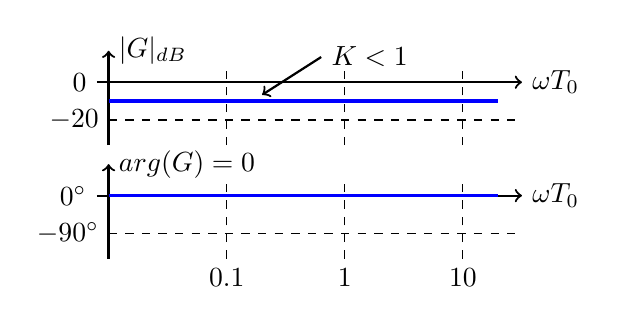
\begin{tikzpicture}[xscale=1.5, yscale=0.8]

%% Amplitude
\begin{scope}
	%% Koordinatensystem
	\draw[thick, ->] (-0.1,0) node[left] {$0$} -- (3.5,0) node[right] {$\omega T_0$};
	\draw[thick, ->] (0,-1) -- (0,0.5) node[right] {$|G|_{dB}$};
	\draw[dashed] (0,-0.6) node[left] {$-20$} -- (3.5,-0.6);
	\draw[dashed] (1,-1) -- +(0,1.2);
	\draw[dashed] (2,-1) -- +(0,1.2);
	\draw[dashed] (3,-1) -- +(0,1.2);
	%%%%%%%%%%%%%%%%

	%% Amplitudengang
	\draw[blue, very thick] (0,-0.3) -- +(3.3,0);
	\draw[<-, thick] (1.3,-0.2) -- +(0.5,0.6) node[right] {$K<1$};
\end{scope}


%% Phase
\begin{scope}[shift={(0,-1.8)}]
	%% Koordinatensystem
	\draw[thick, ->] (-0.1,0) node[left] {$0^\circ$} -- (3.5,0) node[right] {$\omega T_0$};
	\draw[thick, ->] (0,-1) -- (0,0.5) node[right] {$arg(G)=0$};
	\draw[dashed] (0,-0.6) node[left] {$-90^\circ$} -- (3.5,-0.6);
	\draw[dashed] (1,-1) node[below] {$0.1$} -- +(0,1.2);
	\draw[dashed] (2,-1) node[below] {$1$} -- +(0,1.2);
	\draw[dashed] (3,-1) node[below] {$10$} -- +(0,1.2);
	%%%%%%%%%%%%%%%%

	%% Amplitudengang
	\draw[blue, very thick] (0,0) -- +(3.3,0);
\end{scope}

%\draw (current bounding box.south west) rectangle (current bounding box.north east);

\end{tikzpicture}}
	        \\
			\specialrule{2pt}{0pt}{0pt}
			%I-Glied
			I &
			\parbox[c][2cm]{3cm}{\input{./tikzBilder/IGlied}}
			& \begin{minipage}{12cm}
              	$\dot{y} = Ku$\\
              	$u=1(t)$ \hspace{18.5mm} $y=K t$\\
              	$G(j \omega)=\frac{K}{j\omega}$ \hspace{10mm} 
              	$\left| G \right| = \frac{K}{\omega}$ \hspace{10mm}
              	$argG=-\frac{\pi}{2}$\\
              \end{minipage} \rule[-2mm]{0mm}{13mm}
			\\ \cline{2-3}
			& \begin{minipage}{3cm}
	        \includegraphics[angle = {-0.5}, width=3cm]{./bilder/I_Nyq.jpg}
	        \end{minipage}
			& \begin{minipage}{12cm}
	        \includegraphics[angle = {-0.8}, width=8cm]{./bilder/I_Bode.jpg}
	        \end{minipage} \rule[-2mm]{0mm}{30mm}
	        \\
			\specialrule{2pt}{0pt}{0pt}
			%D-Glied
			D &
			\begin{minipage}{3cm}
	        \includegraphics[height=1cm]{./bilder/D_Glied2.png}      \\
	        \includegraphics[angle ={1.7},width=3cm]{./bilder/D_Glied.jpg}
	        \end{minipage}
			& \begin{minipage}{12cm}
              	$y = K\dot{u}$\\
              	$u=1(t)$ \hspace{21.5mm} $y=K \delta (t)$\\
              	$G(j \omega)=K j\omega$ \hspace{10mm} 
              	$\left| G \right| = K\omega$ \hspace{10mm}
              	$argG=\frac{\pi}{2}$\\
              \end{minipage} \rule[-2mm]{0mm}{13mm}
			\\ \cline{2-3}
			& \begin{minipage}{3cm}
	        \includegraphics[angle = {0}, width=3cm]{./bilder/D_Nyq.jpg}
	        \end{minipage}
			& \begin{minipage}{12cm}
	        \includegraphics[angle = {0.5}, width=8cm]{./bilder/D_Bode.jpg}
	        \end{minipage} \rule[-4mm]{0mm}{34mm}
	        \\
			\specialrule{2pt}{0pt}{0pt}
			%PT1_Glied
			$PT_1$ &
			\parbox[c][2cm]{3cm}{\input{./tikzBilder/PT1Glied}}
			& \begin{minipage}{12cm}
              	$T\dot{y}+y=Ku$ \hspace{11.5mm} $y(0)=0$\\
              	$u=1(t)$ \hspace{24mm} $y=K \left[ 1-e^{- \frac{t}{T}}\right]$\\
              	$G(j \omega)= \frac{K}{1+j\omega T}$ \hspace{10mm} 
              	$\left| G \right| = \frac{K}{\sqrt{1+(\omega T)^2}}$
              	\hspace{20mm}
              	$argG=-\arctan(\omega T)$\\
              \end{minipage} \rule[-2mm]{0mm}{13mm}
			\\ \cline{2-3}
			& \begin{minipage}{3cm}
	        \includegraphics[angle = {-0.5}, width=3cm]{./bilder/PT1_Nyq.jpg}
	        \end{minipage}
			& \begin{minipage}{12cm}
	        \includegraphics[angle = {-0.6}, width=8cm]{./bilder/PT1_Bode.jpg}
	        \end{minipage} \rule[-5mm]{0mm}{35mm}
	        \\
			\specialrule{2pt}{0pt}{0pt}
			%PT2_Glied
			$PT_2$ &
			\begin{minipage}{3cm}
	        \includegraphics[width=3cm]{./bilder/PT2_glied.jpg}
	        \end{minipage}
			& \begin{minipage}{12cm}
              	$T^2\ddot{y}+2\zeta T \dot{y}+y=Ku \qquad \text{oder}
              	\qquad	\ddot{y}+2\zeta\omega_n \dot{y}+\omega_n^2y=K\omega_n^2
              	u$\\
              	$y(0)=0$ \hspace{10mm} $\dot{y}(0)=0$ \hspace{10mm}
              	$\omega_n=\frac{1}{T}$\\
              	$y=K \left[1-\frac{1}{\sqrt{1-\zeta^2}}e^{-\zeta\omega_n t}\sin
              	\left( \sqrt{1-\zeta^2} \omega_n t+arcos(\zeta) \right)
              	\right]$\\ 
              	$G(j \omega)= \frac{K}{(j \omega T)^2 + 2 \zeta T (j\omega) + 1}$
              	\hspace{10mm} 
              	$\left| G \right| = \frac{K}{\sqrt{\left[1+(j\omega
              	T)^2\right]^2+\left[2\zeta \omega T \right]^2}}$\\
              	$\arg G=-\arctan  \frac{2\zeta \omega T}{(j\omega T)^2+1}$
              	\hspace{13mm} $0 \leq\omega T \leq 1$\\
              	$\arg G=\arctan \frac{2\zeta \omega T}{(j \omega T)^2+1}-\pi$
              	\hspace{10mm} $1 \leq\omega T \leq \infty$\\
              \end{minipage} \rule[-2mm]{0mm}{22mm}
			\\ \cline{2-3}
			& \begin{minipage}{3cm}
	        \includegraphics[angle = {-0.3}, width=3cm]{./bilder/PT2_Nyq.jpg}
	        \end{minipage}
			& \begin{minipage}{12cm}
	        \includegraphics[angle = {0.2}, width=8cm]{./bilder/PT2_Bode.jpg}
	        \end{minipage} \rule[-5mm]{0mm}{35mm}
	        \\
			\specialrule{2pt}{0pt}{0pt}
			%Tt_Glied
			$T_t$ &
	        \parbox[c][2cm]{3cm}{\input{./tikzBilder/TtGlied}}
			& \begin{minipage}{12cm}
              	$y=\begin{cases}
  				0 & 0<t<T_t \\
  				u(t-T_t) & t \geq T_t
				\end{cases}$\\
              	$u=1(t)$ \hspace{29.5mm} $y=1(t-T_t)$\\
              	$G(j \omega)= e^{-j\omega T_t}$ \hspace{15mm}
              	$\left| G \right| = 1$
              	\hspace{30mm}
              	$argG=-\omega T_t$\\
              \end{minipage} \rule[-2mm]{0mm}{15mm}
			\\ \cline{2-3}
			& \begin{minipage}{3cm}
	        \includegraphics[angle = {0.2}, width=3cm]{./bilder/T_Nyq.jpg}
	        \end{minipage}
			& \begin{minipage}{12cm}
	        \includegraphics[angle = {0.3}, width=8cm]{./bilder/T_Bode.jpg}
	        \end{minipage} \rule[-5mm]{0mm}{35mm}
	        \\
			\specialrule{2pt}{0pt}{0pt}
        \end{longtable}

%----------------------------------------------------------------------------------------
%
%	Tabelle aus Buch Seite 124
%
%
%	\subsection{Der Frequenzgang \formelbuch{117}}
%		\begin{tabular}{| c | c | c | c |}
%		    \hline
%	        $P$-Glied & $I$-Glied & $PT_1$-Glied & $T_t$-Glied \\
%	        \begin{minipage}{3cm}
%	        \includegraphics[width=3cm]{./bilder/pglied}
%	        \end{minipage} &
%			\begin{minipage}{3cm}
%	        \includegraphics[width=3cm]{./bilder/iglied}
%	        \end{minipage} &
%			\begin{minipage}{4cm}
%	        \includegraphics[width=3cm]{./bilder/pt1glied}
%	        \end{minipage} &
%			\begin{minipage}{3cm}
%	        \includegraphics[width=3cm]{./bilder/tglied}
%	        \end{minipage} \\
%	        \hline
%	        $y=Ku$ & $\dot{y} = Ku$ & $T\dot{y}+y = Ku$ & $y=u(t-T_t)$ \\
%	        &  &  & $t\geq T_t$ \\
%	        \hline
%	        $G(j\omega)=K$ & $G(j\omega)= \frac{K}{j\omega}$ &
%	        $G(j\omega)=\frac{K}{1+j\omega T}$ &
%	        $G(j\omega)=e^{-j\omega T_t}$\\
%	        & & & \\
%	        \hline
%	        $\left| G \right| = K$ & $\left| G \right| = \frac{K}{\omega}$ &
%	        $\left| G \right| = \frac{K}{\sqrt{1+(|\omega T)^2}}$ &
%	        $\left| G \right| = 1$ \\
%	        $argG=0$ & $argG= -\frac{\pi}{2}$ & $argG=-\arctan(\omega T)$ &
%	        $argG= - \omega T_t$\\
%	        & & &  \\
%	        \hline
%	        & & & \\
%	        \begin{minipage}{3cm}
%	        \includegraphics[width=2.7cm]{./bilder/fg_pglied}
%	        \end{minipage} &
%			\begin{minipage}{3cm}
%	        \includegraphics[width=3cm]{./bilder/fg_iglied}
%	        \end{minipage} &
%			\begin{minipage}{4cm}
%	        \includegraphics[width=4cm]{./bilder/fg_pt1glied}
%	        \end{minipage} &
%			\begin{minipage}{3cm}
%	        \includegraphics[width=3cm]{./bilder/fg_tglied}
%	        \end{minipage} \\
%			& & & \\
%	        \hline
%	        \end{tabular}

%----------------------------------------------------------------------------------------

	\subsection{Stabilitätsproblem \formelbuch{108}}
		\begin{minipage}{5cm}
		\fbox{$K_I T_t=\frac{\pi}{2}$} \\
		\fbox{$K_I=\omega_\pi$}
		\end{minipage}
		\begin{minipage}{13cm}
        $K_I$: Stabilitätsgrenze \\
        $\omega_\pi$: Phasenschnittfrequenz
        \end{minipage}


	\subsection{Nyquistkriterium \formelbuch{129}}
		Der geschlossene Regelkreis ist genau dann stabil, wenn beim Durchlauf der
		Ortskurve in Richtung zunehmender Frequenz der kritische Punkt -1 \glqq zur
		Linken\grqq\ liegt.
		
	\subsection{Phasenreserve und Verstärkungsreserve \formelbuch{132}}
			\begin{minipage}{3.5cm}
			\fbox{$K_R K_{Rres}=K_{R\pi}$}\\
			\fbox{$K_{Rres}=\frac{1}{\left| G(j\omega_{\pi})\right|}$}\\
			\fbox{$argG_0=-\pi+\Phi_{res}$}\\
			\fbox{$argG_0(\omega_\pi)=-\pi$}\\
			\fbox{$|G_0(j\omega_D)|=1$}\\
			$K_R < K_{R\pi}$\\
			$K_R > K_{R\pi}$	
			\end{minipage}
			\begin{minipage}{9cm}
        	$K_R$: \hspace{5mm}Verstärkung des Reglers \\
        	$K_{Rres}$: Verstärkungsreserve mit Regler (Amplitudenres., gain
        	margin)\\ $K_{R\pi}$: kritische Verstärkung (Verstärkung ohne
        	Regler)\\ $\omega_\pi$: Phasenschnittfrequenz \\
        	$\omega_D$: Durchtrittsfrequenz \\
        	$\Phi_{res}$: Phasenreserve \\ \\ \\
        	Regelung stabil\\
        	Regelung instabil
        	\end{minipage}
			\begin{minipage}{6.2cm}
        		\includegraphics[width=6.2cm]{./bilder/phasenreserve.png}
        	\end{minipage}
			
	\subsection{Sprungantwort und Stabilität \formelbuch{135}}
		\subsubsection{Stabilitätssatz für ein System 2. Ordnung \formelbuch{137}}
			Ein System ist genau dann stabil, wenn {\bf alle} Koeffizienten der
			homogenen Dgl. positiv (oder alle negativ) und ungleich 0 sind.\\
			$\ddot{y}+a_1\dot{y}+a_0y=F(u)$
			
		\subsubsection{Stabilitätssatz für die Sprungantwort}
			Ein LTI-System ist genau dann stabil, wenn die Sprungantwort einem
			konstantem Wert zustrebt.
\newpage
\section{PID-Regler \formelbuch{147}}

	\subsection{P-Regler - Stationärer Zustand \formelbuch{155}}
		Beim einfachsten linearen Regler, dem P-Typ, besteht ein proportionaler
		Zusammenhang zwischen Fehler $e$ und Stellgrösse $u$.\\
		Der P-Regler reagiert schnell, kann aber den Sprungfehler nicht vollständig
		eliminieren. Er hat einen stationären Fehler.
		
	
	\subsection{I-Regler \formelbuch{160}}
		Der reine I-Regler ist allgemein ungünstig, weil er relativ langsam arbeitet
		und die Stabilität schwacht. Ist aber die Regelstrecke nur erster Ordnung
		erziehlt man gute Ergebnisse mit dem I-Regler.\\
		Der I-Regler neigt zum Schwingen.\\
		Bei sprungförmigen Signalen, d.h. für Festwertregelungen hat der I-Regler
		keinen Fehler!
		
	
	\subsection{$PT_2$-Glied \formelbuch{163}}
		\begin{minipage}{5cm}
        \fbox{$T_\omega = 2T_m=\frac{2\pi}{\omega_n \sqrt{1-\zeta
        ^2}}=\frac{2\pi}{\omega}$}\\
        \fbox{$\omega = \frac{2\pi}{T_\omega}=2\pi f$}
        \end{minipage}
		\begin{minipage}{13cm}
        $T_\omega$: Schwingungsdauer\\
        $\omega_n$: Kennkreisfrequenz\\
        $\zeta$: \hspace{1.1mm} Dämpfungskonstante\\
        \end{minipage}\\
		\glqq Optimale Dämpfung\grqq\ bei $\Psi=45$ und $\zeta=\frac{1}{\sqrt{2}}$.
		Dabei erreicht die Regelgrösse $y$ nach $4.3\%$ Überschwingen rasch den
		Endwert.\\
		\begin{minipage}{7cm}
		$T^2\ddot{y}+2\zeta T \dot{y}+ y=Ku$\\
		$\ddot{y}+2\zeta\omega_n\dot{y}+\omega_n^2=\omega_n^2 Ku$
		\end{minipage}
		\begin{minipage}{11cm}
        $\ddot{y}+a_1\dot{y}+a_0 y=\ldots$\\
        $a_1=2\zeta\omega_n$\\
        $a_0=\omega_n^2$
        \end{minipage}
	
	\subsection{PI-Regler \formelbuch{174}}
		\begin{minipage}{15cm}
        \includegraphics[angle={0},width=10cm]{./bilder/PI_Regler.jpg}
        \end{minipage}\\ \\
		\begin{minipage}{15cm}
        \fbox{$G(j\omega)=K_R \frac{1+j\omega T_N}{j\omega T_N}$}\qquad
        \fbox{$arg(G(j\omega))=\arctan(\omega T_N)-\frac{\pi}{2}$}
        \end{minipage}
		
	
	\subsection{D-Glied \formelbuch{179}}
		Der Differenzierer erzeugt eis Korrektursignal im voraus.\\
		Nachteilig ist, wenn die Regelgrösse verrauscht ist, dann werden die
		hochfrequenten Störsignale durch die Ableitung verstärkt.\\
		Ein LTI-System, welches ohne D-Glied darstellbar ist, gegebenenfalls durch
		Umformung des Blockdiagramms, heisst realisierbar.
	
	
	\subsection{PID-Regler \formelbuch{183} \formelbuch{383}}
	\fbox{$G(s) = K_R(1 + \frac{1}{j \omega T_N} + j \omega T_V )$}
	
	\subsection{PD-Regler \formelbuch{187} \formelbuch{383}}
	\fbox{$u=K_R at+K_R T_V a$} \qquad
	Das PD-Glied entspricht dem inversen PT$_1$-Glied.
	
	\subsection{Empirische Einstellregeln \formelbuch{188}}
		\includegraphics[width=13cm]{./bilder/Empirisch_Regeln.jpg}
		\begin{minipage}[b]{5cm}
        UTF des angenäherten Modells:\\ \\
		$G_0(j\omega)=\frac{K_s}{1+j\omega T_g}e^{-j\omega T_u}$
		\vspace{2.7cm}
		\end{minipage}\\
		
	\begin{tabular}{|l|p{1.8cm}|l|l|l|l||l|l|}
	    \hline
	    \multicolumn{6}{|c||}{
	      \textbf{Reglereinstellung nach Chien-Hrones-Reswick}
	    } &
	    \multicolumn{2}{|c|}{
	      \textbf{Reglereinstellung nach Ziegler-Nichols}
	    }
		\\ \hline
		\multicolumn{6}{|c||}{
		  $
		  q = \frac{T_g}{T_uK_S} \qquad \mu = \frac{T_g}{T_u}
		  \qquad \text{wenn} \quad \mu
		  \begin{cases}
		    > 10 \rightarrow \text{Strecke gut regelbar} \\
		    < 3 \rightarrow \text{Strecke schlecht regelbar}
		  \end{cases}
		  $
		} & $q=\frac{T_g}{T_uK_s}$ & $K_{R\pi} \qquad T_\pi=\frac{2\pi}{\omega_\pi}$
		\\ \hline
		\textbf{Regler} & \textbf{Regler\-parameter} &
		\multicolumn{2}{|p{3.5cm}|}{\textbf{Führungsverhalten} \newline $y_m$:
		Überschwingen} &
		\multicolumn{2}{|c||}{\textbf{Störverhalten}} &
		\textbf{Sprungantwort} & \textbf{Stabilitätsgrenze}
		\\ \hline
		& & kein $y_m$ & $\frac{y_m}{y_\infty} = 20 \%$ & kein $a$ & $\frac{a}{b}= 20 \%$ & & 
		\\ \hline
		P 	& $K_R$ 	& $0.3q$ 	& $0.7q$ 	& $0.3q$ 	& $0.7q$	& $q$ 	& $0.5K_{R\pi}$ 
		\\ \hline
		PI	& $K_R$		& $0.35q$	& $0.6q$	& $0.6q$	& $0.7q$	& $0.9q$ 	& $0.45K_{R\pi}$
		\\
		    & $T_N$		& $1.17T_g$	& $1T_g$	& $4T_u$	& $2.33T_u$ & $3.33T_u$ & $0.85T\pi$
		\\ \hline
		PID & $K_R$		& $0.6q$	& $0.95q$	& $0.95q$	& $1.2q$ 	& $1.2q$ 	& $0.60K_{R\pi}$
		\\
			& $T_N$		& $1T_g$	& $1.36T_g$	& $2.38T_u$	& $2T_u$ 	& $2T_u$	& $0.50T\pi$
		\\
			& $T_V$		& $0.5T_u$	& $0.47T_u$	& $0.42T_u$	& $0.42T_u$ & $0.5T_u$ 	& $0.125T_\pi$
		\\ \hline
	\end{tabular}
	
		
	\subsection{Wind-Up \formelbuch{200}}
		Die Folge eines \glqq wind-up-Phänomens\grqq\ ist einerseits ein konstanter
		Fehler und anderseits eine verzögert reagierende und damit stark überschwingende
		Regelgrösse.\\ \\
		\underline{wind-up entsteht durch:}\\
		\begin{itemize}
		\item bestehender Fehler
		\item I-Anteil im Regler
		\item Sättigung der Stellgrösse
		\end{itemize}
		

\section{Diverses}
	\subsection{Frequenzgang zweier Systeme mit Rückkopplung }
			\begin{center}
        		\includegraphics[height=3cm]{./bilder/feedback.png}
        	\end{center}

	\subsection{Graphisch Phasen-/Verstärkungsreserve}
		\includegraphics[width=7cm]{./bilder/bode-stabilitaet.png} \\
		Phasen-/Verstärkungsreserve = Phasen-/Amplitudenrand
		

\end{document}
